\section{Results}

\subsection{25 Vertices}

When applied to a random graph with 25 vertices, the genetic algorithm finds a nicely optimized solution after 100 iterations, with a mutation rate of .5, a crossover rate of 1, and 100 chromosomes.

\begin{figure}[H]
\centering
\begin{tabular}{cccccc}
\subfloat[Step 2]{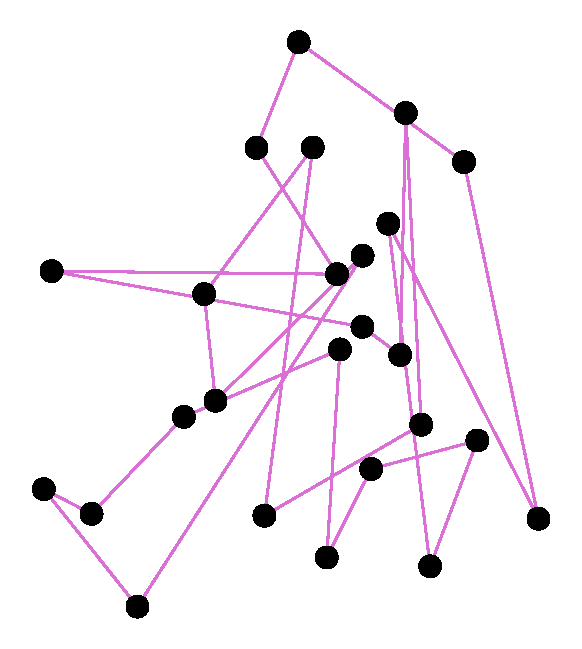
\includegraphics[width = .75in]{images/25/vis_2.pdf}} &
\subfloat[Step 10]{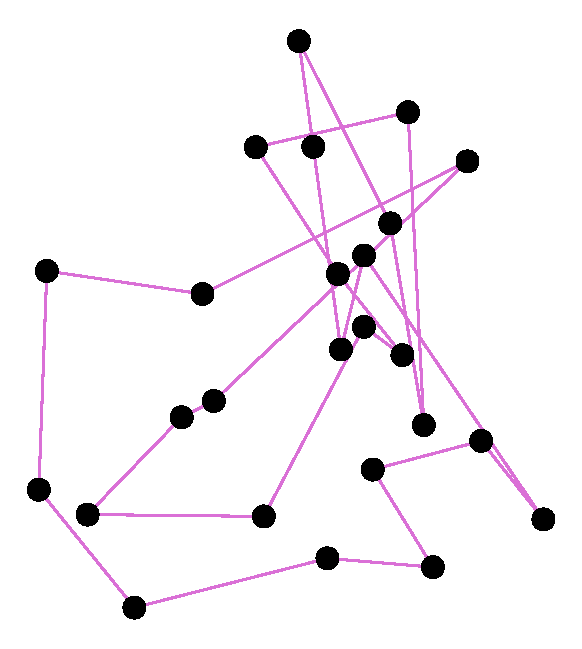
\includegraphics[width = .75in]{images/25/vis_10.pdf}} &
\subfloat[Step 20]{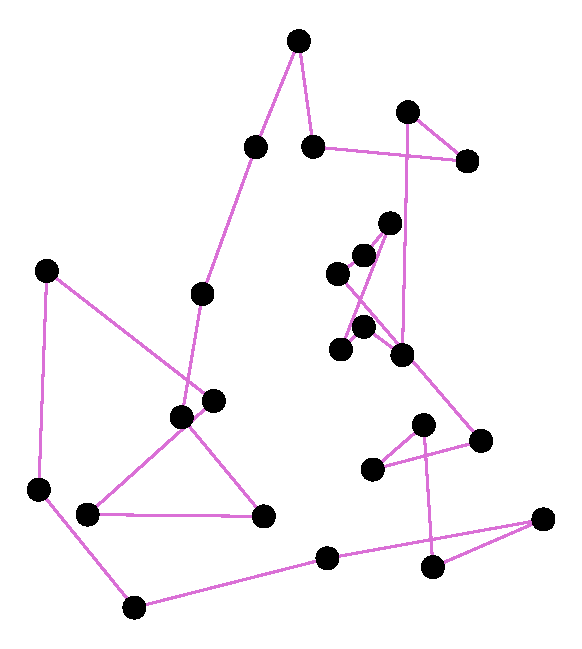
\includegraphics[width = .75in]{images/25/vis_20.pdf}} &
\subfloat[Step 30]{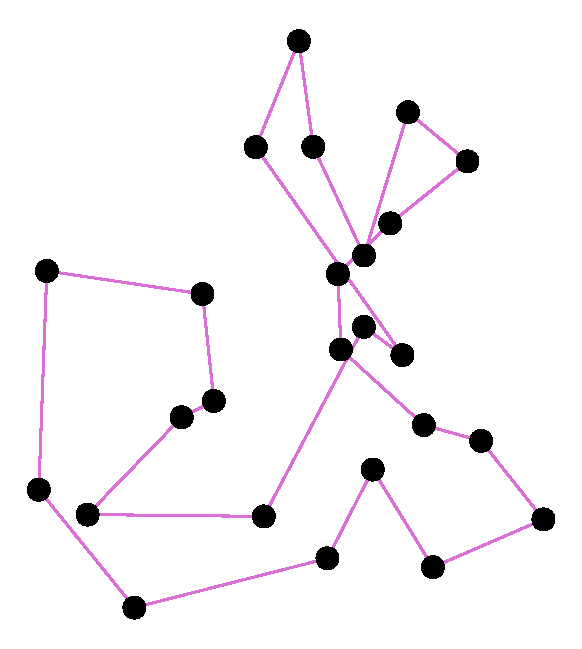
\includegraphics[width = .75in]{images/25/vis_30.pdf}} &
\subfloat[Step 40]{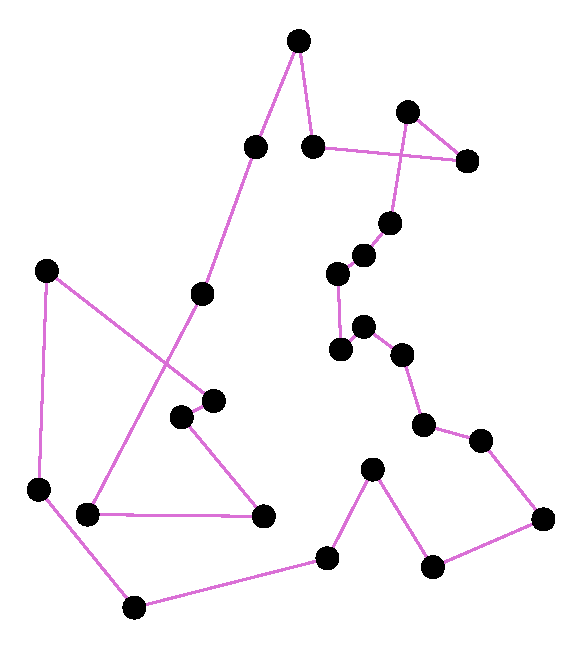
\includegraphics[width = .75in]{images/25/vis_40.pdf}} \\
\subfloat[Step 50]{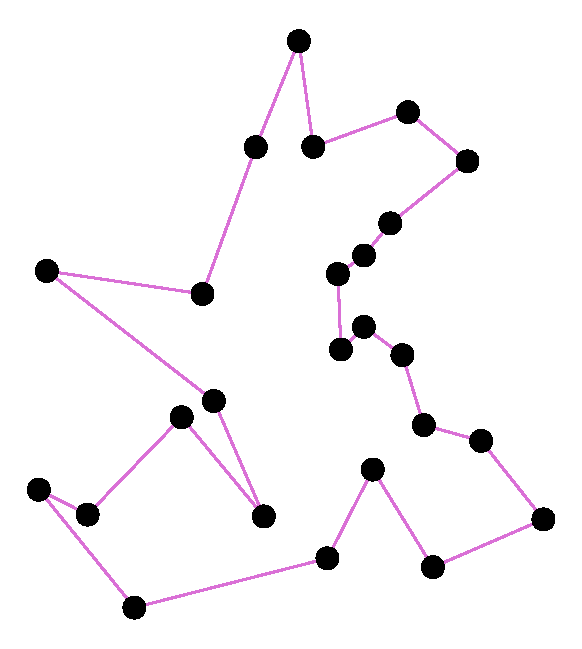
\includegraphics[width = .75in]{images/25/vis_50.pdf}} &
\subfloat[Step 60]{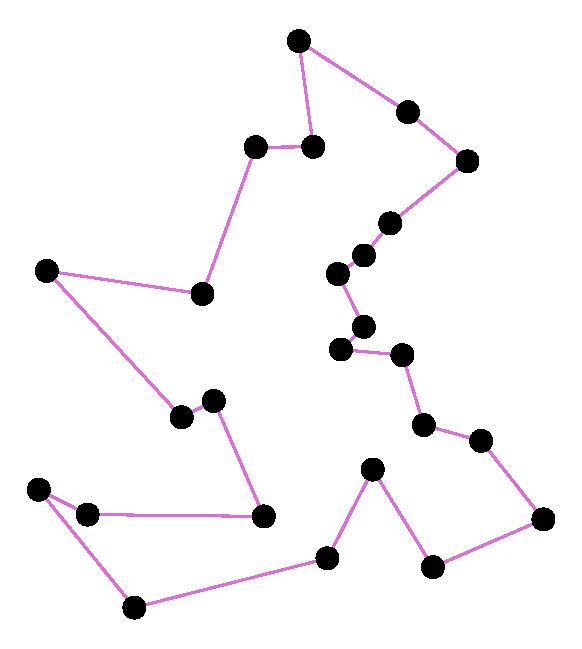
\includegraphics[width = .75in]{images/25/vis_60.pdf}} &
\subfloat[Step 70]{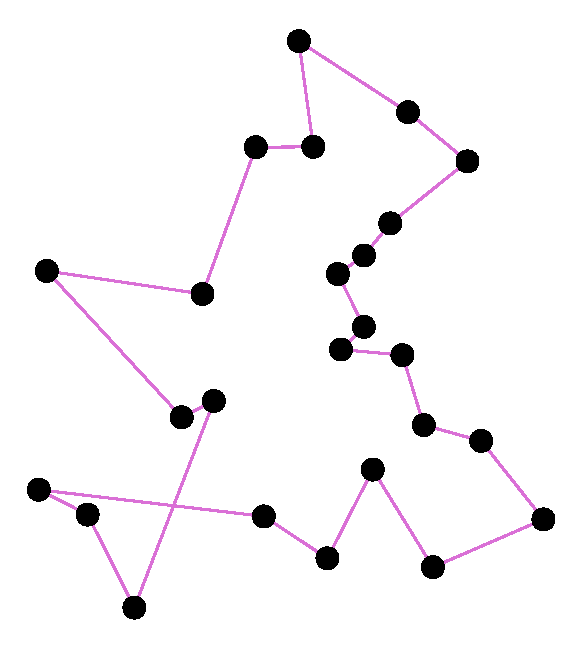
\includegraphics[width = .75in]{images/25/vis_70.pdf}} &
\subfloat[Step 80]{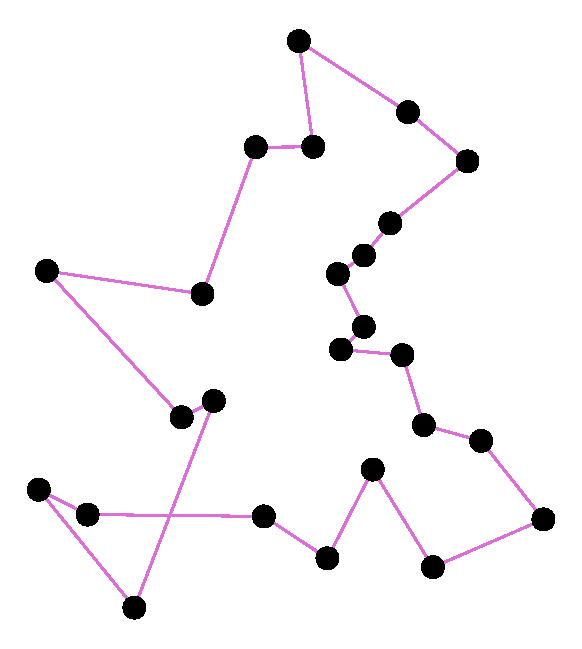
\includegraphics[width = .75in]{images/25/vis_80.pdf}} &
\subfloat[Step 90]{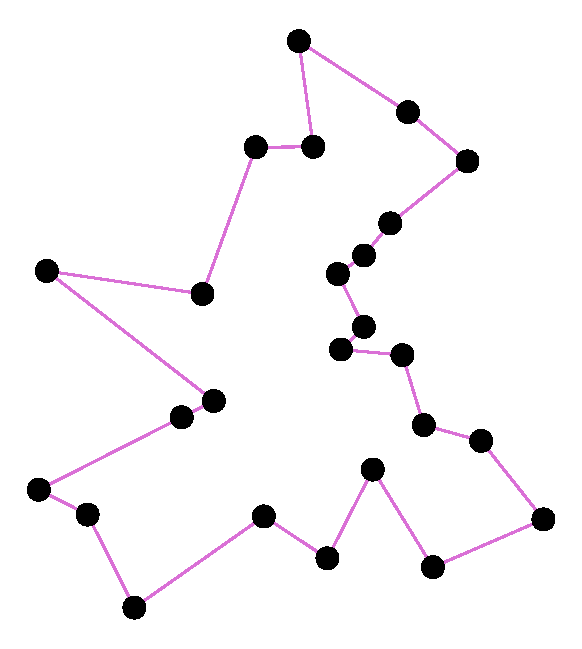
\includegraphics[width = .75in]{images/25/vis_90.pdf}} \\

\end{tabular}
\caption{The genetic algorithm working on an algorithm with 25 vertices.}
\end{figure}

\begin{figure}[H]
\centering
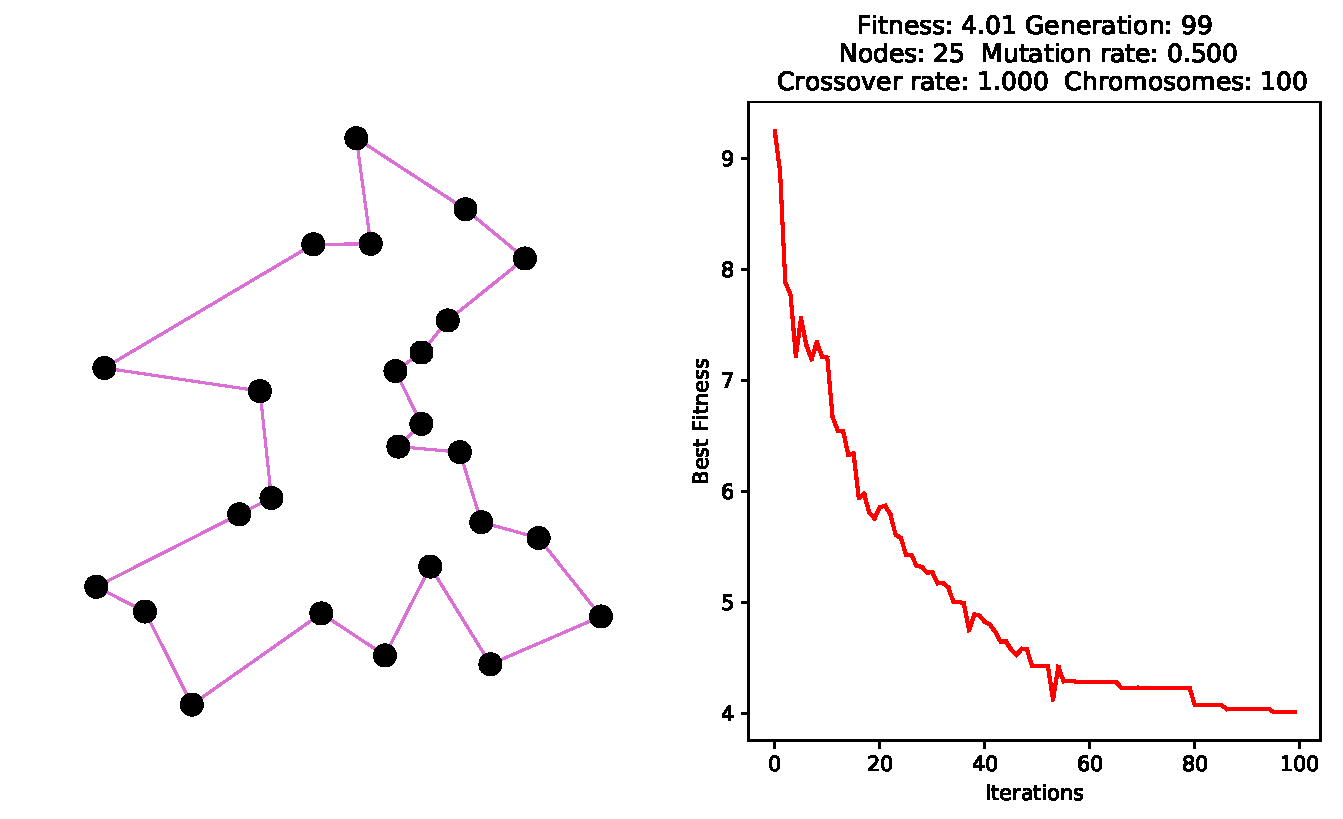
\includegraphics[width=6in]{images/25/graph_100.pdf}
\caption{The genetic algorithm working on a random graph with 25 nodes after 100 iterations.}
\label{fig:somthing}
\end{figure}

For this example, the genetic algorithm begins with a random solution with fitness of 23 distance units. After 138 iterations, the fittest solution has 7.28 distance units, a 3x improvements.

\subsection{100 Verticess}

At 100 vertices, the algorithm takes longer to optimize, but is able to optimize from 45 distance units in the first iteration to 10.42 in the 625th generation, an improvement of 4.5x.

\begin{figure}[H]
\centering
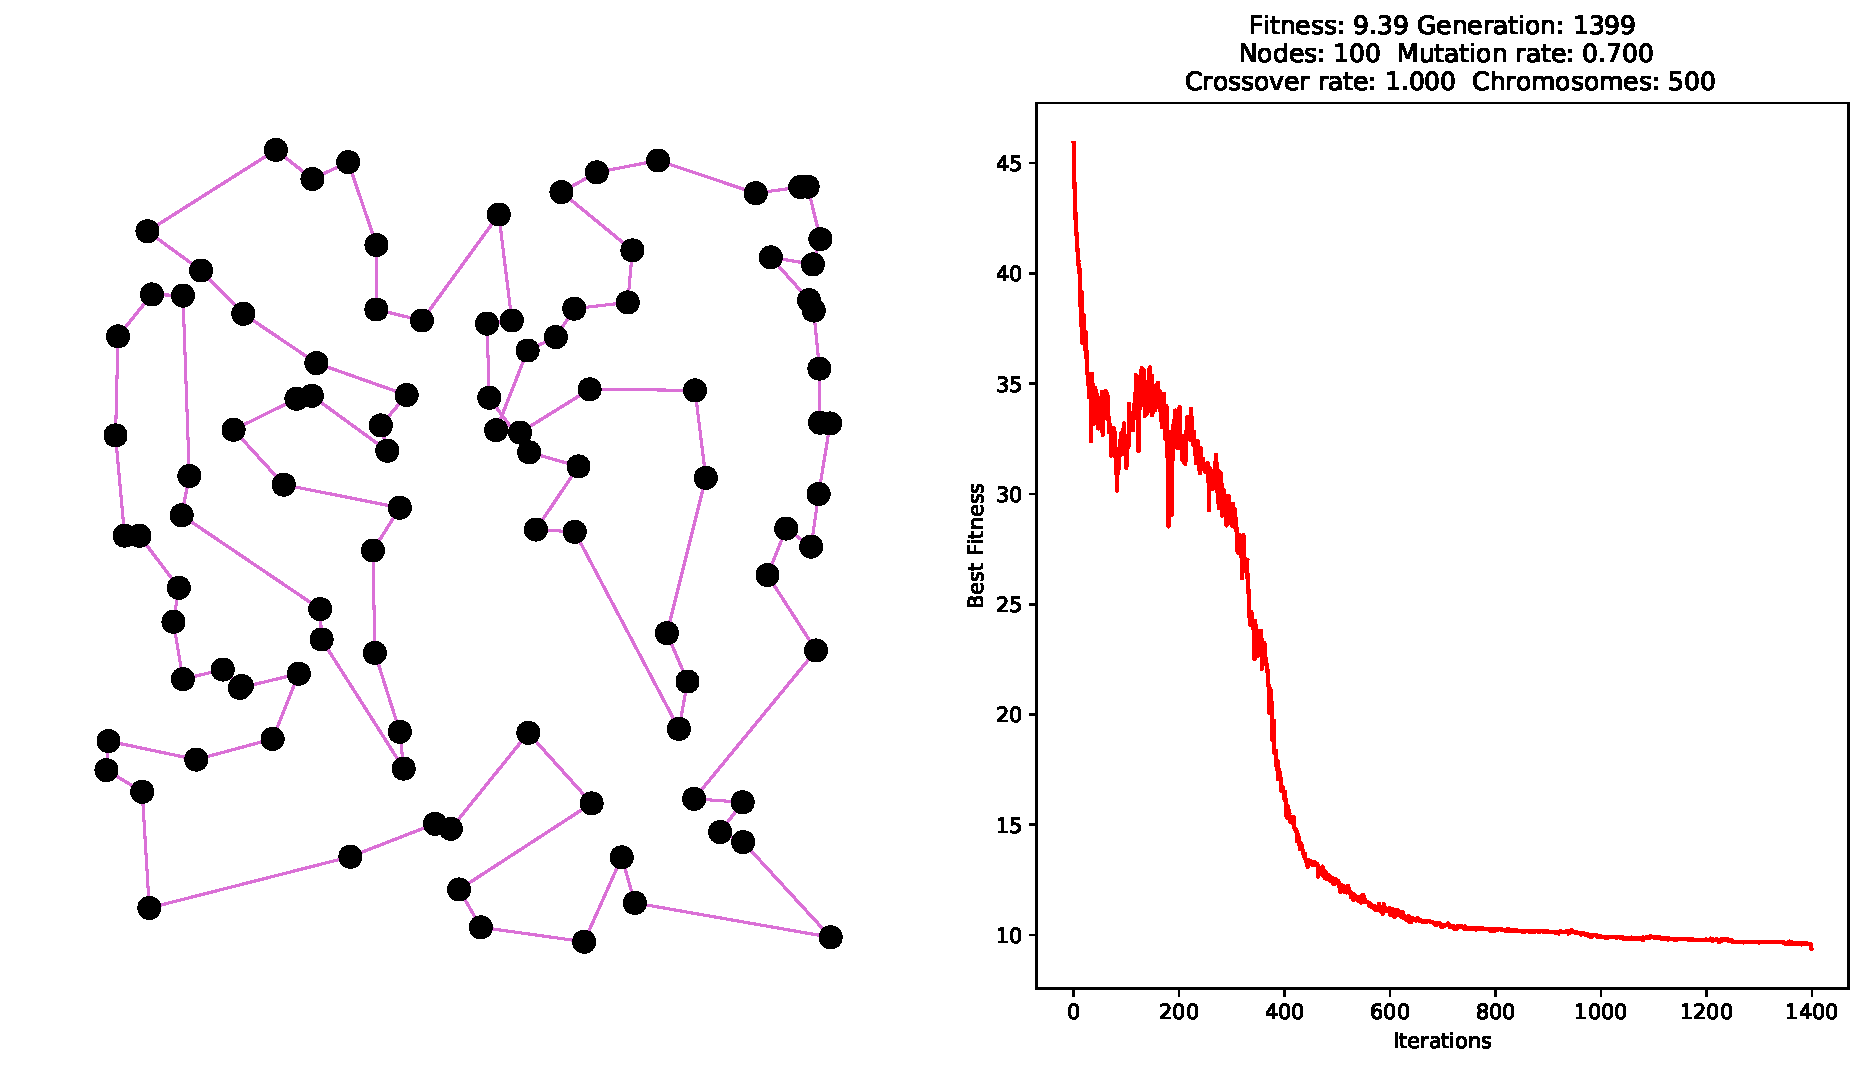
\includegraphics[width=6in]{images/100.pdf}
\caption{The genetic algorithm applied to a graph of 100 random vertices.}
\label{fig:somthing}
\end{figure}

\subsection{Real-world Dataset}

A great litmus test is a real-world dataset. This dataset is 128 of the largest cities in North America.

\begin{figure}[H]
\centering
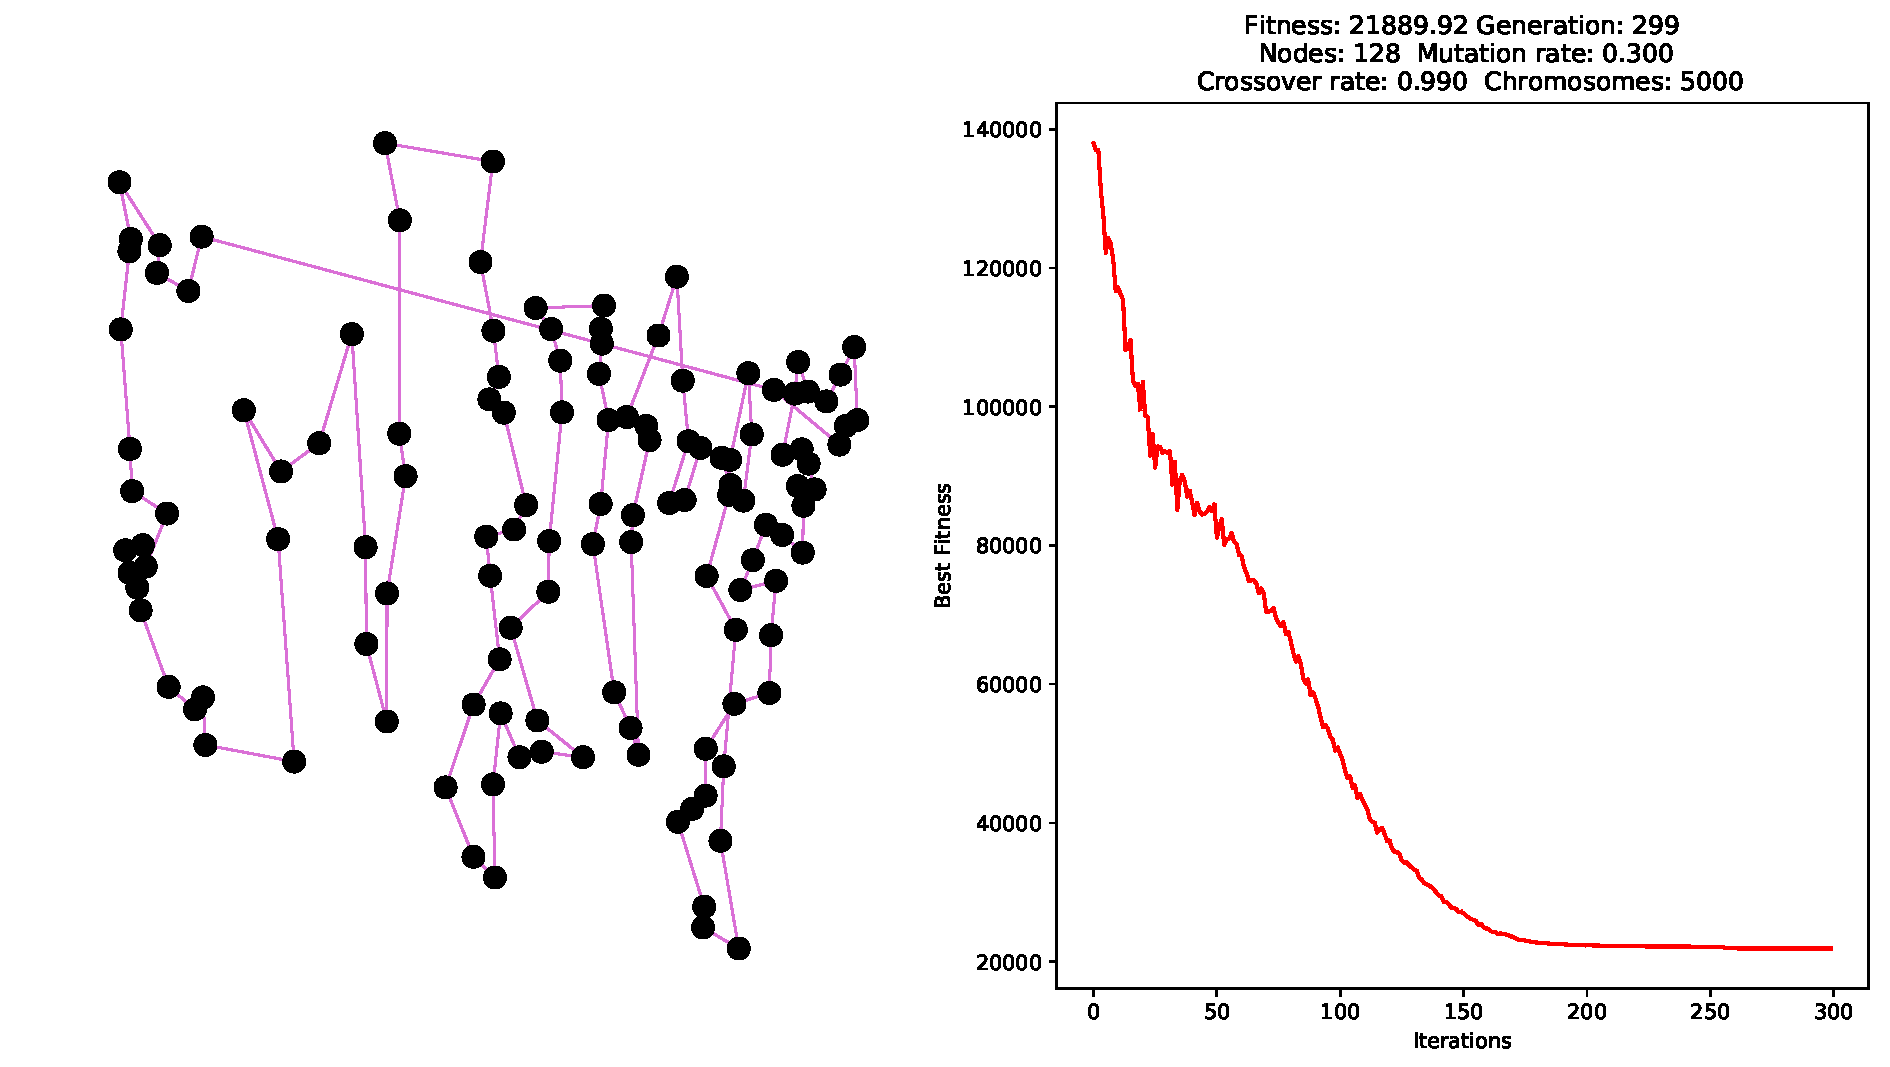
\includegraphics[width=6in]{images/north_america.pdf}
\caption{The genetic algorithm applied to an XY projection of 128 major cities in North America.}
\label{fig:somthing}
\end{figure}